Si prova innanzitutto la macchina sull'insieme di dati \emph{Iris},
tipicamente utilizzato per testare i classificatori.

Ne risulta un tasso di successo anche del 100\% (\textsc{Figura~\ref{fig:iris100}}).

\begin{figure}
  \centering
  \resizebox{.9\textwidth}{!}{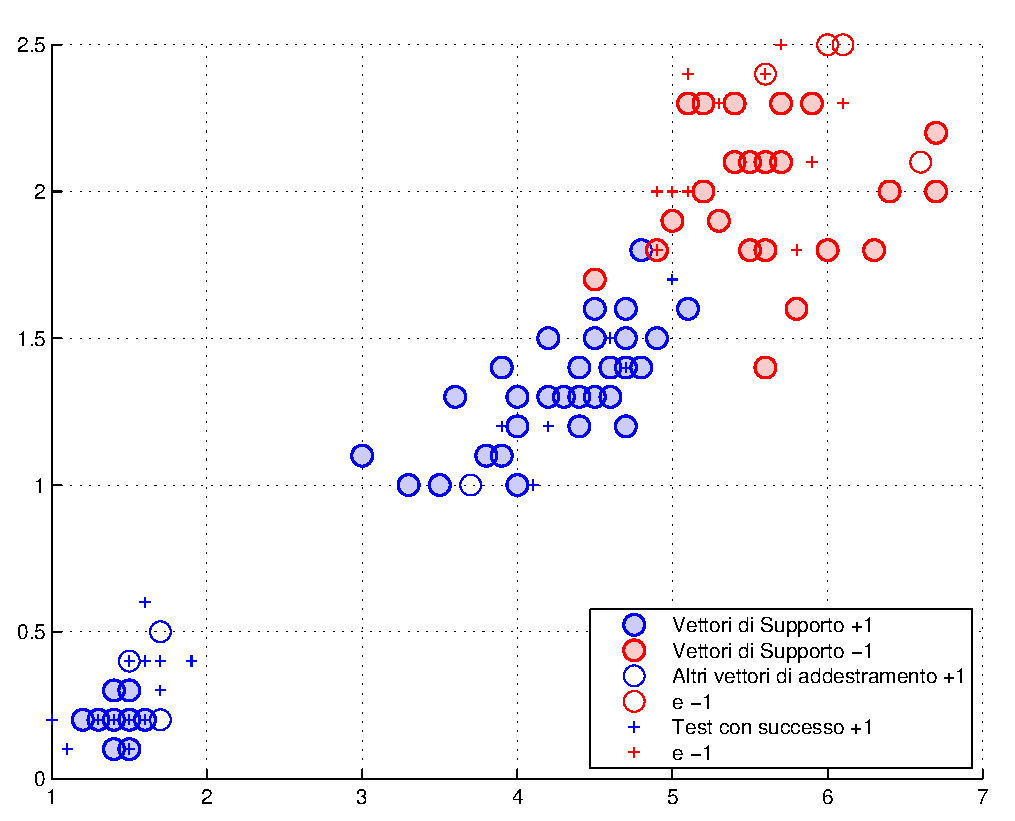
\includegraphics{Disegni/Iris100}}
  \caption{La \ac{svm} testata sul \textit{Iris} ottiene un tasso di successo fino al 100\%.}
  \label{fig:iris100}
\end{figure}

La si addestra poi seguendo i protocolli proposti in letteratura
e lo si collauda su un insieme di test.

Le risposte fornite dalla macchina sono confrontate con i giudizi dell'esperta.